\begin{surferPage}{Чмутова површ осмог степена}
    Оно што визуелно привлачи Чмутовој површи осмог степена  $\text{Chm}_{d}, \ d=8 $
    јесте њена симетрија.
    Она се може претпоставити анализирањем њене једначине:
    \[\text{Chm}_{d}\colon T_d(x) + T_d(y) + T_d(z) + 1 = 0,\]
     где је $T_d$ такозвани Чебишевљев полином (слика лево).
    Крива $T_8(x)+T_8(y)=0$ је представљена десно:
    
     \begin{center}
      \begin{tabular}{c@{\quad}c}
        \begin{tabular}{c}
          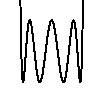
\includegraphics[height=1.75cm]{./../../common/images/Tcheb_008.pdf}
        \end{tabular}    
        &
        \begin{tabular}{c}
          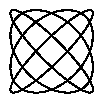
\includegraphics[height=1.75cm]{./../../common/images/Tcheb_2d_008.pdf}
        \end{tabular}    
      \end{tabular}
    \end{center}
    \vspace{-0.3cm}
    Корак од ових слика до облика површи на интерактивној слици није дугачак.


Ове једначине је поставио С. В. Чмутов раних 80-тих година.
    У то време оне су биле светски рекорд.
    Деведесетих година Чмутов је поправио сопствени рекорд а 2005. су 
    Бреске, Лабс и ван Стратен прерадили ову конструкцију и добили реалне 
	површи са реалним сингуларитетима.
\end{surferPage}
